\labeledsection{Reinforcement Learning}{sec:rl}
\titledbox{Motivation}{
\begin{itemize}
    \item \linkterm{Supervised Learning}{supervised_learning} trains an agent on explicit, labeled target outputs
    \item \linkterm{Unsupervised Learning}{unsupervised_learning} extracts hidden patterns or structures from unlabeled data without any external guidance or feedback.
    \item \defemph{Reinforcement Learning} is a distinct paradigm where an agent learns through trial-and-error interaction with a dynamic environment, guided only by a scalar reward signal.
    \item For example, in chess, the agent learns a strategy (\defemph{policy}) to maximize the chance of winning by evaluating the outcomes of its moves, rather than relying on pre-recorded grandmaster games.
\end{itemize}
}

\anondefinition{
A \defemph{reinforcement} is a scalar feedback value (reward signal) returned by the environment that quantifies the immediate success or failure of an agent's action.
}{reinforcement}

\Example{
In soccer, the agent receives positive reinforcement for scoring goals and maintaining possession, and negative reinforcement for conceding goals or receiving penalties.
}{}

\anondefinition{
\defemph{Reinforcement Learning} is a machine learning paradigm where an \linkterm{agent}{def:agent} learns to map situations to actions so as to maximize a cumulative numerical reward signal, without being explicitly told which actions to take.
}{reinforcement_learning}

\titledbox{Remember}{
We introduced \linkterm{rewards}{MDP} as parts of \linkterm{MDPs}{MDP}. An \linkterm{optimal policy}{optimal_policy_mdp} maximizes the expected total \linkterm{reward}{MDP}.
}

\redbox{
The task of \linkterm{Reinforcement Learning}{reinforcement_learning} is to use the observed \linkterm{rewards}{MDP} to come up with an \linkterm{optimal policy}{optimal_policy_mdp}
}

\commandnote{
In \linkterm{MDPs}{MDP}, the \linkterm{agent}{def:agent} has total knowledge about the environment and the \linkterm{reward function}{MDP}, in \linkterm{Reinforcement Learning}{reinforcement_learning} we do not assume this. \linkterm{Reinforcement Learning}{reinforcement_learning} $\approx$ \linkterm{POMDP}{pomdp} but with \linkterm{reward}{MDP}-learning.
}


\titledbox{For Simplicity}{
    We focus exclusively on simple environments and basic agent designs:
    \begin{itemize}
        \item \textbf{Passive Learning:} A \linkterm{utility-based agent}{utility_based_agent} learns a \linkterm{utility function}{utility_based_agent} over states, using it to select actions that maximize the \linkterm{expected utility}{expected_utility}.
        \item \textbf{Active (Q-Learning):} A Q-learning agent learns an action-utility function (Q-function) that provides the \linkterm{expected utility}{expected_utility} of executing a specific action in a given state.
        \item \textbf{Policy Learning:} A \linkterm{reflex agent}{def:reflex} learns a \linkterm{policy}{policy} that maps states directly to corresponding actions.
    \end{itemize}
}

\begin{align*}
\textbf{Utility-based agent (Passive):} \quad & \text{state} \rightarrow \text{utility} \\
\textbf{Q-learning agent (Active):} \quad & \text{state} + \text{action} \rightarrow \text{expected utility} \\
\textbf{Reflex agent (Direct):} \quad & \text{state} \rightarrow \text{action}
\end{align*}

\anondefinition{
\defemph{Passive Learning} is where an \linkterm{agent}{def:agent} uses a state-based representation in a \linkterm{fully observable}{env_types} environment with a fixed \linkterm{policy}{policy} $\pi$. The goal is to evaluate the quality of this policy by learning the \linkterm{utility function}{utility_based_agent} $U^{\pi}(s)$, which determines the \linkterm{expected utility}{expected_utility} of executing action $\pi(s)$ in state $s$.
}{passive_learning}

\commandnote{
\linkterm{Passive Learning}{passive_learning} is similar to \linkterm{policy evaluation}{policy_iteration} which is part of the \linkterm{policy iteration}{policy_iteration} algorithm. However, the agent here \textbf{does not} know 
\begin{itemize}
    \item the \linkterm{transition model}{transition_model_hmm} $P(s' \mid s, a)$
    \item the \linkterm{reward function}{MDP} $R(s)$
\end{itemize}
}

\Example{
We use the $4 \times 3$ grid world introduced previously:
\begin{figure}[H]
    \centering
    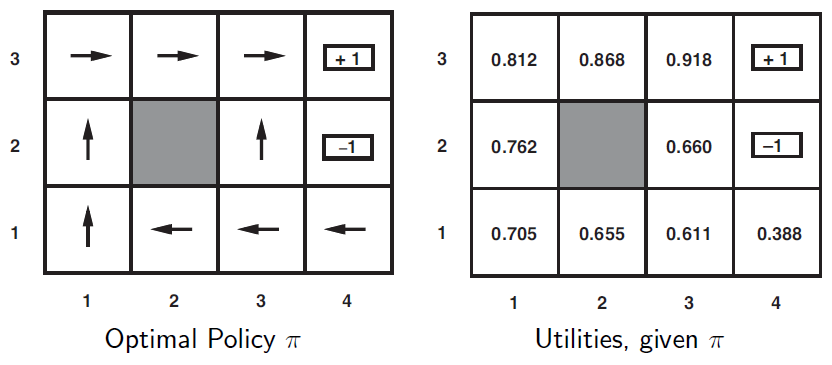
\includegraphics[width=0.5\linewidth]{images/rl_example_grid.png}
\end{figure}
\begin{itemize}
    \item The \linkterm{agent}{def:agent} executes a \linkterm{set}{def:set} of trials in the environment using its \linkterm{policy}{policy} $\pi$
    \item In each trial, the \linkterm{agent}{def:agent} starts in state $(1,1)$ and experiences a \linkterm{sequence}{sequence} of state transitions until it reaches one of the terminal states $(4,2)$ or $(4,3)$
    \item Its percepts supply both the current state and the \linkterm{reward}{MDP} received in that state
\end{itemize}
}{}

\Example{
The trials might look like this: 
\begin{enumerate}
\item $(1,1)_{-0.04} \leadsto (1,2)_{-0.04} \leadsto (1,3)_{-0.04} \leadsto (1,2)_{-0.04} \leadsto (1,3)_{-0.04} \leadsto (2,3)_{-0.04} \leadsto (3,3)_{-0.04} \leadsto (4,3)_{+1}$
\item $(1,1)_{-0.04} \leadsto (1,2)_{-0.04} \leadsto (1,3)_{-0.04} \leadsto (2,3)_{-0.04} \leadsto (3,3)_{-0.04} \leadsto (3,2)_{-0.04} \leadsto (3,3)_{-0.04} \leadsto (4,3)_{+1}$
\item $(1,1)_{-0.04} \leadsto (2,1)_{-0.04} \leadsto (3,1)_{-0.04} \leadsto (3,2)_{-0.04} \leadsto (4,2)_{-1}$
\end{enumerate}
}{trials_passive}

\anondefinition{
In \linkterm{Passive Learning}{passive_learning}, the \defemph{utility} is defined to be the expected sum of \linkterm{discounted rewards}{discounted_rewards} obtained if \linkterm{policy}{policy} $\pi$ is followed:
\[
U^{\pi}(s) := \mathbb{E} \left[ \sum_{t=0}^{\infty} \gamma^t R(S_t) \right]
\]
where $R(s)$ is the \linkterm{reward}{MDP} for a state $s$, $S_t$ (a \linkterm{random variable}{def:random_variable}) is the state reached at time $t$ when executing \linkterm{policy}{policy} $\pi$ and $S_0 = s$
}{utility_rl_passive}

\commandnote{
We assume no \linkterm{discounted rewards}{discounted_rewards} for simplicity \hfill ($\gamma = 1$)
}

\definition{Reward-to-Go}{
The \linkterm{utility}{utility_rl_passive} of a state is the expected total \linkterm{reward}{MDP} from that state onward
}{reward_to_go}

\ideabox{
Each trial provides a sample of the \linkterm{reward-to-go}{reward_to_go} for each state visited
}

\Example{
Consider the first trial from \Exampleref{trials_passive}:
\[
(1,1)_{-0.04}
\leadsto
(1,2)_{-0.04}
\leadsto
(1,3)_{-0.04}
\leadsto
(1,2)_{-0.04}
\leadsto
(1,3)_{-0.04}
\leadsto
(2,3)_{-0.04}
\leadsto
(3,3)_{-0.04}
\leadsto
(4,3)_{+1}
\]

Since we assume no discounting ($\gamma = 1$), the \linkterm{reward to go}{reward_to_go} is simply the sum of all rewards from the current state until the terminal state.

For state $(1,1)$:
\[
-0.04 -0.04 -0.04 -0.04 -0.04 -0.04 -0.04 + 1
=
1 - 7(0.04)
=
0.72
\]

Thus, the trial provides a sample utility of $0.72$ for $(1,1)$.

The state $(1,2)$ is visited twice:
\[
-0.04 -0.04 -0.04 -0.04 -0.04 -0.04 + 1
=
0.76
\]
and
\[
-0.04 -0.04 -0.04 -0.04 + 1
=
0.84
\]

Hence, the trial provides two utility samples for $(1,2)$: $0.76$ and $0.84$.

Similarly, the state $(1,3)$ is visited twice:
\[
-0.04 -0.04 -0.04 -0.04 -0.04 + 1
=
0.80
\]
and
\[
-0.04 -0.04 -0.04 + 1
=
0.88
\]

Thus, the trial provides two utility samples for $(1,3)$: $0.80$ and $0.88$.

In general, every visit to a state yields one sample of its \linkterm{utility}{utility_rl_passive}. Averaging these samples over many trials gives an estimate of $U^{\pi}(s)$.
}{}

\anondefinition{
The \defemph{direct utility estimation} algorithm cycles over trials, calculates the \linkterm{reward-to-go}{reward_to_go} for each state, and updates the estimated utility for that state by keeping the running average for that for each state in a table
}{direct_utility_estimation}

\observationbox{
In the limit, the sample average will converge ot the true expectation (\linkterm{utility}{utility_rl_passive}) from \Defref{utility_rl_passive}
}

\Example{
We illustrate \linkterm{direct utility estimation}{direct_utility_estimation} over multiple trials.

Assume we track utilities for two states $s_1$ and $s_2$.

\textbf{Trial 1:}
\begin{itemize}
    \item $s_1 \rightarrow$ reward-to-go: $0.70$
    \item $s_1 \rightarrow$ reward-to-go: $0.74$
    \item $s_2 \rightarrow$ reward-to-go: $0.80$
\end{itemize}

After Trial 1:
\[
\hat U(s_1) = \frac{0.70 + 0.74}{2} = 0.72,
\quad
\hat U(s_2) = 0.80
\]

\textbf{Trial 2:}
\begin{itemize}
    \item $s_1 \rightarrow$ reward-to-go: $0.68$
    \item $s_2 \rightarrow$ reward-to-go: $0.82$
    \item $s_2 \rightarrow$ reward-to-go: $0.78$
\end{itemize}

Now we use \textbf{all samples seen so far}:

For $s_1$:
\[
\hat U(s_1) = \frac{0.70 + 0.74 + 0.68}{3} = 0.7067
\]

For $s_2$:
\[
\hat U(s_2) = \frac{0.80 + 0.82 + 0.78}{3} = 0.80
\]

\textbf{Trial 3:}
\begin{itemize}
    \item $s_1 \rightarrow$ reward-to-go: $0.75$
    \item $s_2 \rightarrow$ reward-to-go: $0.77$
\end{itemize}

After Trial 3:

For $s_1$:
\[
\hat U(s_1) = \frac{0.70 + 0.74 + 0.68 + 0.75}{4} = 0.7175
\]

For $s_2$:
\[
\hat U(s_2) = \frac{0.80 + 0.82 + 0.78 + 0.77}{4} = 0.7925
\]

\textbf{Summary:} each new trial adds more \linkterm{reward-to-go}{reward_to_go} samples, and the utility estimate is always the running average over all samples seen so far.
}{}

\observationbox{
\linkterm{Direct utility estimation}{direct_utility_estimation} is just \linkterm{supervised learning}{supervised_learning} where each \linkterm{example}{supervised_learning} has the state as input and the observed \linkterm{reward-to-go}{reward_to_go} as output
}

\problembox{
The main issue with \linkterm{direct utility estimation}{direct_utility_estimation} is that it ignores the fact that state utilities are structurally linked through the dynamics of the environment. It incorrectly treats the value of each state as something that can be learned independently from raw returns.

\begin{itemize}
    \item In reality, the utility of a state is not an isolated quantity, but depends on the utilities of successor states reached under the policy.
    \item This creates strong dependencies between state values: changing the estimate of one state affects the correct value of others.
\end{itemize}
}

\redbox{
The utility values are in fact constrained by the \linkterm{Bellman Equation}{bellman_equation} for a fixed \linkterm{policy}{policy} $\pi$, which enforces consistency between all states:
\[
U^{\pi}(s) = R(s) + \gamma \cdot \left( \sum_{s'} P(s' \mid s, \pi(s)) \cdot U^{\pi}(s') \right)
\]

This shows that the value of a state is defined recursively in terms of the values of successor states, meaning all utilities must be solved jointly rather than independently.
}

\titledbox{Intuition}{
\linkterm{Direct utility estimation}{direct_utility_estimation} searches for $U$ in a \linkterm{hypotheses space}{supervised_learning} that is too large $\leadsto$ many \linkterm{functions}{function} that violate the \linkterm{Bellman Equation}{bellman_equation} $\leadsto$ thus the algorithm often converges slowly
}

\ideabox{
Take advantage of the constraints among the utilities of states by:
\begin{itemize}
    \item learning the \linkterm{transition model}{transition_model_hmm} that connects them,
    \item solving the corresponding \linkterm{MDP}{MDP} using a dynamic programming approach
\end{itemize}
This mean plugging the learned \linkterm{transition model}{transition_model_hmm} $P(s' \mid s, \pi(s))$ and the observed \linkterm{rewards}{MDP} $R(s)$ into the \linkterm{Bellman Equation}{bellman_equation} to calculate the utilities of the states
}

\titledbox{Remember}{
These equations are linear (no maximization involved) $\leadsto$ solve with any linear algebra package
}

\observationbox{
Learning the model itself is easy, because the environment is \linkterm{fully observable}{env_types}
}
\Corollary{
We have a \linkterm{supervised learning}{supervised_learning} task where the input is a state-action pair and the output is the resulting state 
\begin{itemize}
    \item In the simplest case, we can represent the \linkterm{transition model}{transition_model_hmm} as a table of probabilities
    \item Count how often each action outcome occurs and estimate the \linkterm{transition probability}{transition_model_hmm} $P(s' \mid s, a)$ from the frequency with which $s'$ is reached by action $a$ in $s$
\end{itemize}
}{}

\Example{
In the 3 trials from \Exampleref{trials_passive}, \texttt{Right} is executed 3 times in $(1,3)$ and 2 times the result is $(2,3)$, so $P((2,3) \mid (1,3) , \texttt{Right})$ is estimated to be $\frac{2}{3}$
}{}

\titledbox{ADP}{
Adaptive Dynamic Programming (ADP) does the idea we are talking about. It first learns how the world behaves (transition probabilities), then uses that learned model to solve the Bellman equations and compute utilities.

Instead of \textit{"average observed returns"} (\linkterm{direct utility estimation}{direct_utility_estimation}) it does build model $\to$ plug into \linkterm{Bellman Equation}{bellman_equation} $\to$ compute utilities consistently 
}

\anondefinition{
A \defemph{Passive ADP agent} first learns an explicit \linkterm{transition model}{transition_model_hmm} $P(s' \mid s, \pi(s))$ and a reward model $R(s)$ from experience, and then computes the \linkterm{utility function}{utility_based_agent} by solving the \linkterm{Bellman Equation}{bellman_equation} for the fixed policy $\pi$.
}{passive_adp}

\commandnote{
The idea is: instead of estimating utilities directly from sampled returns, ADP enforces consistency by using the learned environment model to solve for utilities globally via the Bellman equations.
}

\titledbox{Active Reinforcement Learning}{
\begin{itemize}
    \item In \linkterm{Passive Learning}{passive_learning}, the agent follows a fixed \linkterm{policy}{policy} and only evaluates it.
    \item In \textbf{Active Reinforcement Learning}, the agent must both learn from experience and decide which actions to take in the environment.
    \item This means the agent is no longer evaluating a given policy, but is instead trying to discover an \linkterm{optimal policy}{optimal_policy_mdp}.
\end{itemize}
}

\ideabox{
We extend the idea of a \linkterm{Passive ADP agent}{passive_adp}: instead of only evaluating a fixed policy, the agent learns a full transition model for all actions and uses it to compute an optimal policy.
}

\begin{itemize}
    \item The agent learns a complete model of the environment, i.e. $P(s' \mid s, a)$ for all actions $a$, not just those chosen by a fixed policy.
    
    \item It uses this model to compute the optimal utility function, which satisfies the \linkterm{Bellman optimality equation}{bellman_equation}:
    \[
    U(s) = R(s) + \gamma \cdot \max_{a \in \mathcal{A}_s} \sum_{s'} P(s' \mid s, a)\, U(s')
    \]

    \item The resulting utilities are used to derive a policy via \linkterm{value iteration}{value_iteration} or \linkterm{policy iteration}{policy_iteration}.

    \item Action selection is typically done by one-step look-ahead:
    \[
    a = \arg\max_a \sum_{s'} P(s' \mid s, a)\, U(s')
    \]
\end{itemize}

\observationbox{
A greedy active ADP agent selects actions that are optimal with respect to its current learned model. However, since the model is incomplete or inaccurate, the resulting policy may be suboptimal in the true environment.
}

\questionbox{
What should the agent do, given that it does not have access to the true environment model and must learn it through interaction?
}

\ideabox{
Actions serve a dual purpose beyond receiving immediate rewards under the current model:
\begin{itemize}
    \item They generate new experience that improves the learned \linkterm{transition model}{transition_model_hmm} by influencing the observations the agent receives.
    \item A better model leads to improved decision-making, which can increase future cumulative \linkterm{rewards}{MDP}.
\end{itemize}
}

\observationbox{
The agent must balance two competing objectives:
\begin{itemize}
    \item \refterm{exploitation}{exploitation}: selecting actions that maximize immediate performance according to the current estimate of the \linkterm{utility function}{utility_based_agent}.
    \item \refterm{exploration}{exploration}: selecting actions that improve knowledge of the environment in order to achieve higher long-term performance.
\end{itemize}
}

\commandnote{
Pure \linkterm{exploitation}{exploitation} can trap the agent in suboptimal behavior due to incomplete knowledge, while pure \linkterm{exploration}{exploration} fails if the acquired knowledge is never used to optimize behavior.
}



